\section{Zener Diode as a Regulator}

Zener diode có một điện áp đánh thủng ngược được xác định rõ ràng, tại đó nó bắt đầu dẫn điện và tiếp tục hoạt động liên tục trong chế độ phân cực nghịch mà không bị hỏng. Ngoài ra, điện áp rơi qua diode vẫn giữ nguyên trong một phạm vi rộng của các mức điện áp, đặc điểm này khiến diode Zener phù hợp để sử dụng trong các bộ chỉnh áp.

\begin{figure}[H]
    \centering
    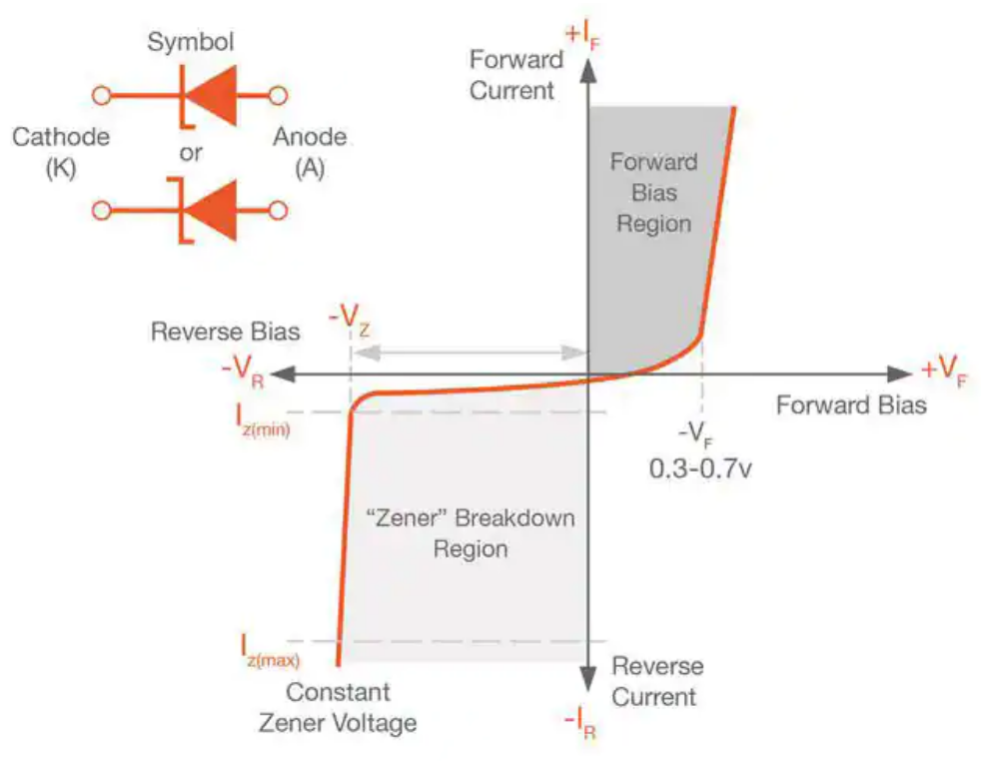
\includegraphics[width=0.8\textwidth]{graphics/ex8/f1.png}
    \caption{Đặc tính điện của Zener diode}
\end{figure}
\clearpage
Trong bài tập này, một Zener diode được dùng để tạo một mạch chỉnh áp có sơ đồ nguyên lý như sau:

\begin{figure}[H]
    \centering
    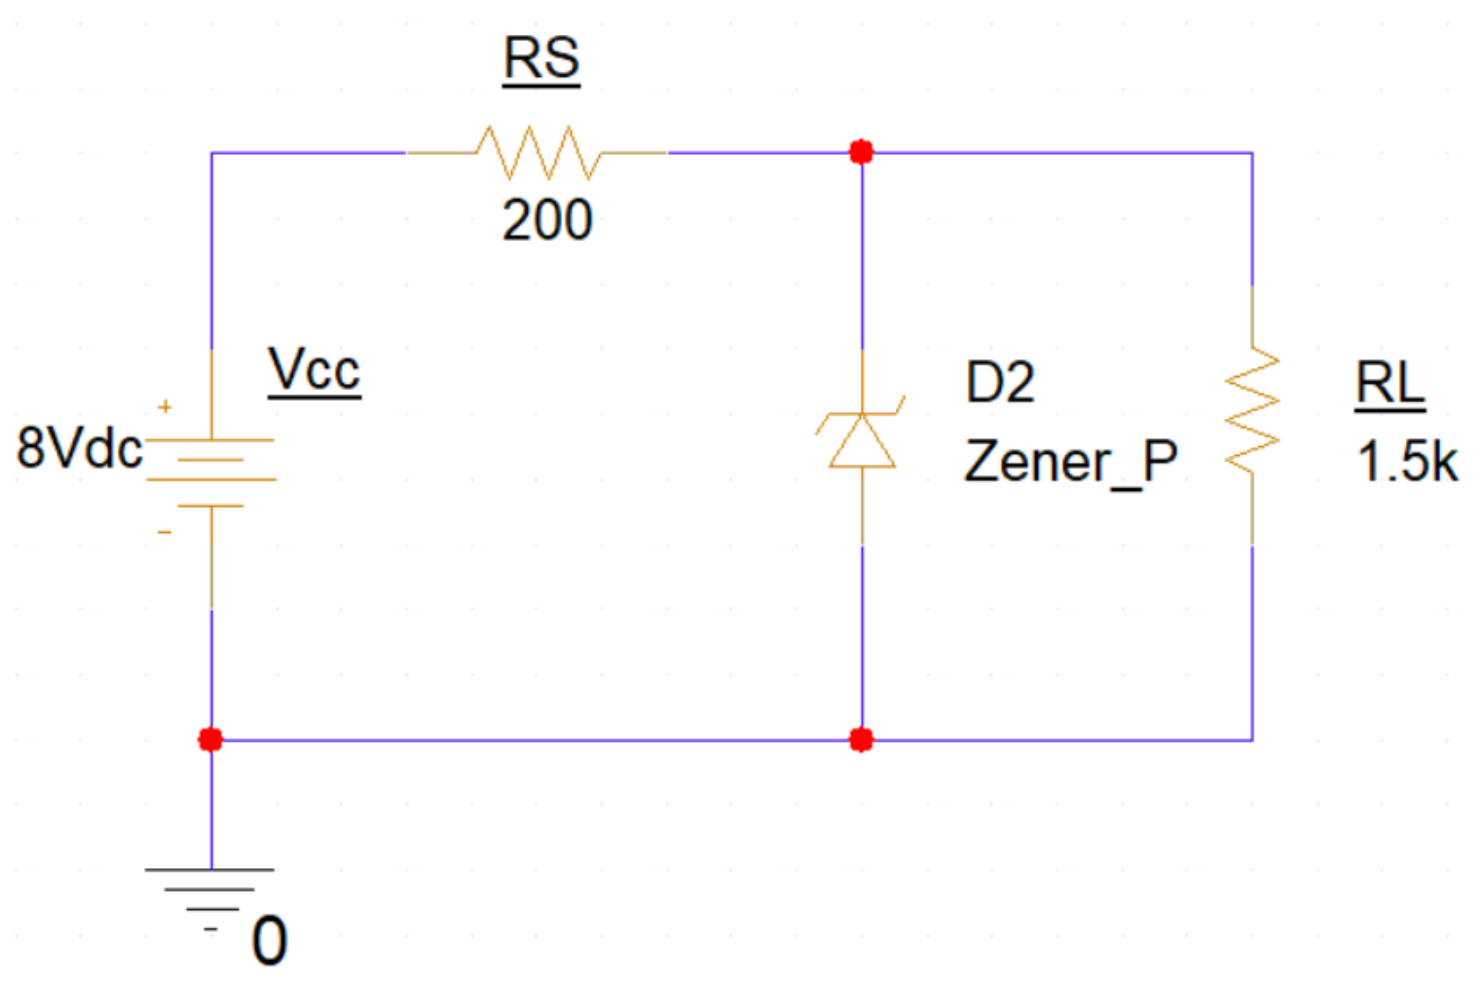
\includegraphics[width=0.8\textwidth]{graphics/ex8/f2.png}
    \caption{Mạch chỉnh áp sử dụng Zener diode}
\end{figure}

\textit{Đoạn này giữ nguyên văn tiếng Anh để dễ thao tác trên PSpice:}

The Zener component in the circuit can be found in the Favourites list by searching the keyword \textbf{Zener}. The full name of the component used in the circuit above is \textbf{Zener\_P - Zener Diode (parameterized)}. The default Zener voltage of this component is $V_{Z} = 5V$. However, this value can be changed in the properties of the component (right click and select Edit Properties) for other simulations.
% Lưu ý cực kỳ quan trọng: khi dùng đoạn văn bản có ký hiệu đặc biệt, phải tách nó ra dùng cặp dấu $...$  ; cái nữa đó là muốn viết Zener_P thì phải ghi code Zener\_P
\subsection{Thành lập công thức tính cho các đại lượng}
\begin{itemize}
    \item \(I_{L} = \frac{V_{L}}{R_{L}} = \frac{V_{Z}}{R_{L}}\) (dựa vào $R_{L} // Z$)
    \item \(I_{S} = \frac{V_{S}}{R_{S}} = \frac{Vcc - V_{Z}}{R_{S}}\) (dựa vào KVL: $Vcc = V_{S} + V_{Z}$) 
    \item \(I_{Z} = I_{S} - I_{L}\) (dựa vào KCL $I_{S} = I_{Z} + I_{L}$)
    \item \(P_{RS} = V_{S} \cdot I_{S} = (Vcc - V_{Z}) \cdot I_{S}\)
    \item \(P_{Z} = V_{Z} \cdot I_{Z}\)
\end{itemize}

\subsection{Tính toán các đại lượng trên trong 2 trường hợp}
\subsubsection{Khi nguồn cấp là 8V}
\begin{itemize}
    \item \(I_{L} = \frac{V_{L}}{R_{L}} = \frac{V_{Z}}{R_{L}} =\frac{5V}{1.5k\Omega} = 3.33mA\)
    \item \(I_{S} = \frac{V_{S}}{R_{S}} = \frac{Vcc - V_{Z}}{R_{S}} = \frac{8V - 5V}{200\Omega} = 15mA\)  
    \item \(I_{Z} = I_{S} - I_{L} = 15mA - 3.33mA = 11.67mA\) 
    \item \(P_{RS} = V_{S} \cdot I_{S} = (Vcc - V_{Z}) \cdot I_{S} = (8V - 5V) \cdot 15mA = 45mW\)
    \item \(P_{Z} = V_{Z} \cdot I_{Z} = 5V \cdot 11.67mA = 58.35mW\)
\end{itemize}
\subsubsection{Khi nguồn cấp là 12V}
\begin{itemize}
    \item \(I_{L} = \frac{V_{L}}{R_{L}} = \frac{V_{Z}}{R_{L}} = \frac{5V}{1.5k\Omega} = 3.33mA\) 
    \item \(I_{S} = \frac{V_{S}}{R_{S}} = \frac{Vcc - V_{Z}}{R_{S}} = \frac{12V - 5V}{200\Omega} = 35mA\) 
    \item \(I_{Z} = I_{S} - I_{L} = 35mA - 3.33mA = 31.67mA\) 
    \item \(P_{RS} = V_{S} \cdot I_{S} = (Vcc - V_{Z}) \cdot I_{S} = (12V - 5V) \cdot 35mA = 245mW\)
    \item \(P_{Z} = V_{Z} \cdot I_{Z} = 5V \cdot 31.67mA = 158.35mW\)
\end{itemize}
\subsection{Mô phỏng trên PSpice}
\begin{figure}[H]
    \centering
    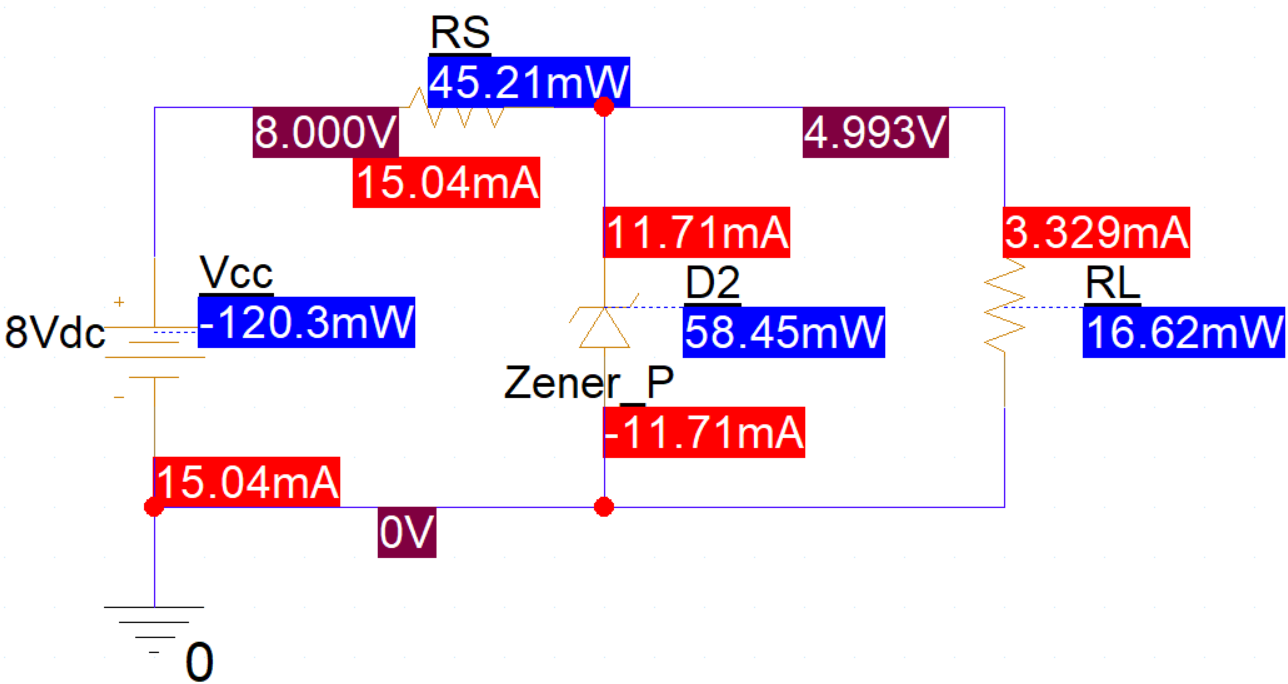
\includegraphics[width=1\textwidth]{graphics/ex8/f3.png}
    \caption{Mạch chỉnh áp với nguồn 8V}
\end{figure}

\begin{figure}[H]
    \centering
    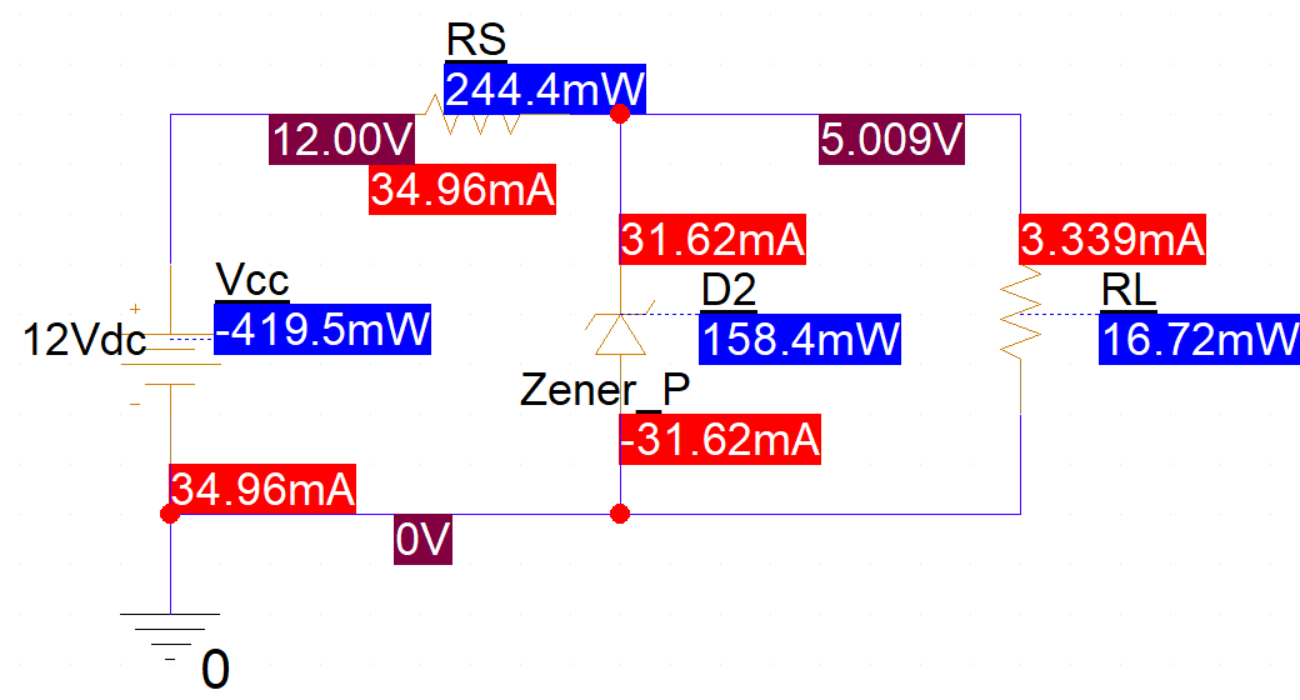
\includegraphics[width=1\textwidth]{graphics/ex8/f4.png}
    \caption{Mạch chỉnh áp với nguồn 12V}
\end{figure}

\subsection{So sánh kết quả tính toán và mô phỏng}
Bảng dưới đây là bảng tổng hợp các số liệu dựa trên tính toán lý thuyết và mô phỏng.
\begin{table}[H]
    \centering
    \begin{tabular}{|c|c|c|c|c|c|c|c|c|c|c|c|c|}
        \cline{2-13}
        \multicolumn{1}{c|}{} & \multicolumn{6}{c|}{\textbf{Tính toán theo lý thuyết}} & \multicolumn{6}{c|}{\textbf{Mô phỏng PSpice}} \\ \cline{2-13}
        \multicolumn{1}{c|}{} & $I_{S}$ & $I_{L}$ & $I_{Z}$ &$V_{L}$ &$P_{RS}$ & $P_{Z}$ & $I_{S}$ & $I_{L}$ & $I_{Z}$ &$V_{L}$ & $P_{RS}$ & $P_{Z}$ \\ \hline
        $Vcc = 8V$ & \makecell{ 15\\ mA} & \makecell{ 3.33\\ mA} & \makecell{ 11.67\\ mA} & \makecell{ 5\\ V} & \makecell{ 45\\ mW} & \makecell{ 58.35\\ mW} & \makecell{15.04 \\ mA} & \makecell{3.329 \\ mA} & \makecell{11.71 \\ mA} & \makecell{4.993 \\ V} & \makecell{45.21 \\ mW} & \makecell{58.45 \\ mW} \\ \hline
        $Vcc = 12V$ & \makecell{ 35\\ mA} & \makecell{ 3.33\\ mA} & \makecell{ 31.67\\ mA} & \makecell{ 5\\ V} & \makecell{ 245\\ mW} & \makecell{ 158.35\\ mW} & \makecell{34.96\\ mA} & \makecell{3.339\\ mA} & \makecell{31.62\\ mA} & \makecell{ 5.009\\ V} & \makecell{244.4 \\ mW} & \makecell{ 158.4\\ mW} \\ \hline
    \end{tabular}
\end{table}